\documentclass[tikz]{standalone}
\usepackage{tikz}
\usetikzlibrary{arrows, calc, positioning, shapes.arrows, decorations.markings}

\tikzstyle{riscv_stage}=[rectangle,draw=black, align=center]
\tikzstyle{fenn_stage}=[rectangle,draw=black, align=center]
\tikzstyle{pipeline_arrow}=[single arrow, draw=gray!75, minimum height=5mm,
                            outer sep=0pt, single arrow tip angle=110]
\tikzstyle{vec_arrow} = [thick, decoration={markings,mark=at position
   1 with {\arrow[semithick]{open triangle 60}}},
   double distance=1.4pt, shorten >= 5.5pt,
   preaction = {decorate},
   postaction = {draw,line width=1.4pt, white,shorten >= 4.5pt}]
\tikzstyle{inner_white} = [semithick, white,line width=1.4pt, shorten >= 4.5pt]
\tikzstyle{invisible} = [inner sep=0,minimum size=0]
\begin{document}
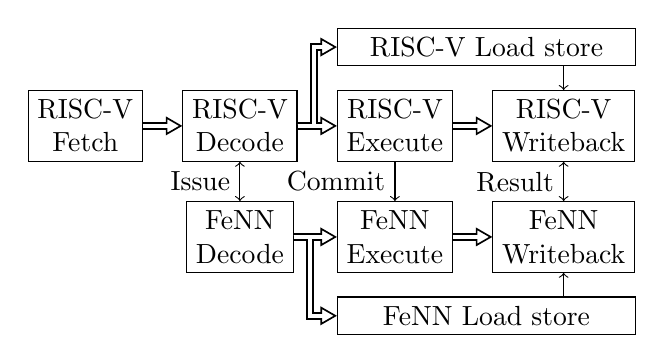
\begin{tikzpicture}


% RISC-V stages
\node [riscv_stage] (scalar_fetch)                                          {RISC-V\\Fetch};
\node [riscv_stage] (scalar_decode)         [right=5mm of scalar_fetch]     {RISC-V\\Decode};
\node [invisible]   (scalar_decode_ex)      [right=2mm of scalar_decode]    {};
\node [riscv_stage] (scalar_ex)             [right=5mm of scalar_decode]    {RISC-V\\Execute};
\node [riscv_stage] (scalar_wb)             [right=5mm of scalar_ex]        {RISC-V\\Writeback};

\path let
    \p1 = (scalar_ex.west),
    \p2 = (scalar_wb.east),
    \n1 = {\x2-\x1} in
    node [riscv_stage] (scalar_lsu)  [above=3mm of scalar_ex.north west, 
                                      anchor=south west,
                                      minimum width=\n1]  {RISC-V Load store};

% RISC-V writeback data
\draw [<-] (scalar_wb.north) to (scalar_wb.north |- scalar_lsu.south);

% RISC-V pipeline arrow
\draw[vec_arrow] (scalar_fetch) to (scalar_decode);
\draw[vec_arrow] (scalar_decode_ex) |- (scalar_lsu);
\draw[vec_arrow] (scalar_decode) to (scalar_ex);
\draw[vec_arrow] (scalar_ex) to (scalar_wb);

% 2nd pass to tidy branching arrows
\draw[inner_white] (scalar_decode) to (scalar_ex);
\draw[inner_white] (scalar_decode_ex) |- (scalar_lsu);

% FeNN stages and XIF interface signals
\node [fenn_stage] (vector_decode)     [below=5mm of scalar_decode]    {FeNN\\Decode}
    edge [<->] node[auto]{Issue} (scalar_decode.south);
\node [invisible] (vector_decode_ex)      [right=2mm of vector_decode]    {};
\node [fenn_stage] (vector_ex)    [below=5mm of scalar_ex]   {FeNN\\Execute}
    edge [<-] node[auto]{Commit} (scalar_ex.south);
\node [fenn_stage] (vector_wb)  [below=5mm of scalar_wb]  {FeNN\\Writeback}
    edge [<->] node[auto]{Result} (scalar_wb.south);

\path let
    \p1 = (vector_ex.west),
    \p2 = (vector_wb.east),
    \n1 = {\x2-\x1} in
    node [fenn_stage] (vector_lsu)  [below=3mm of vector_ex.south west, 
                                     anchor=north west,
                                     minimum width=\n1]  {FeNN Load store};

% FeNN writeback data
\draw [<-] (vector_wb.south) to (vector_wb.south |- vector_lsu.north);

% FeNN pipeline arrows
\draw[vec_arrow] (vector_decode) to (vector_ex);
\draw[vec_arrow] (vector_ex) to (vector_wb);
\draw[vec_arrow] (vector_decode_ex) |- (vector_lsu);

% 2nd pass to tidy branching arrows
\draw[inner_white] (vector_decode) to (vector_ex);
\draw[inner_white] (vector_decode_ex) |- (vector_lsu);
 
% TODO draw dotted horizontal line
% TODO subtly colour lines

\end{tikzpicture}
\end{document}
